\documentclass{article}
\usepackage{tikz}
\usetikzlibrary{arrows.meta}

\begin{document}

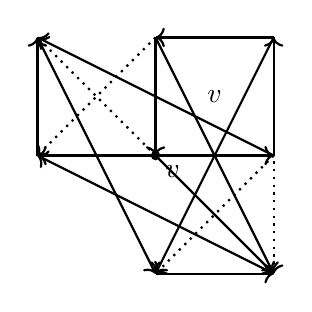
\begin{tikzpicture}[scale=1.5]
    % Define coordinates
    \coordinate (A) at (0,0);
    \coordinate (B) at (1,0);
    \coordinate (C) at (1,1);
    \coordinate (D) at (0,1);
    \coordinate (E) at (-1,0);
    \coordinate (F) at (-1,1);
    \coordinate (G) at (0,-1);
    \coordinate (H) at (1,-1);

    % Draw the vertices
    \filldraw[black] (A) circle (1pt) node[below right] {$v$};
    \filldraw[white] (B) circle (1pt);
    \filldraw[white] (C) circle (1pt);
    \filldraw[white] (D) circle (1pt);
    \filldraw[white] (E) circle (1pt);
    \filldraw[white] (F) circle (1pt);
    \filldraw[white] (G) circle (1pt);
    \filldraw[white] (H) circle (1pt);

    % Draw the edges
    \draw[thick,->] (A) -- (B);
    \draw[thick,->] (B) -- (C);
    \draw[thick,->] (C) -- (D);
    \draw[thick,->] (D) -- (A);
    \draw[thick,->] (A) -- (E);
    \draw[thick,->] (B) -- (F);
    \draw[thick,->] (C) -- (G);
    \draw[thick,->] (D) -- (H);
    \draw[thick,->] (E) -- (F);
    \draw[thick,->] (F) -- (G);
    \draw[thick,->] (G) -- (H);
    \draw[thick,->] (H) -- (E);

    % Draw the dotted lines
    \draw[dotted, thick, ->] (A) -- (F);
    \draw[dotted, thick, ->] (B) -- (G);
    \draw[dotted, thick, ->] (C) -- (H);
    \draw[dotted, thick, ->] (D) -- (E);

    % Draw the solid line
    \draw[thick, ->] (A) -- (H);

    % Label the vertices
    \node at (0.5, 0.5) {$v$};
\end{tikzpicture}

\caption{Result from Example~\ref{ex:facefan2} with \( H_{-v}^{max} \) (solid line) and \( H_{-v}^{min} \) (dashed).}
\label{fig:facefan2}

\end{document}